% Carried over verbatim from monograph/main.tex (Study 1 record, 13 Sep 2026).
\chapter{System architecture and fail-closed philosophy}\label{s1:ch:ch05_system_architecture_and_fail_closed_phil}

\section{Pipeline}

\begin{figure}[H]
\centering
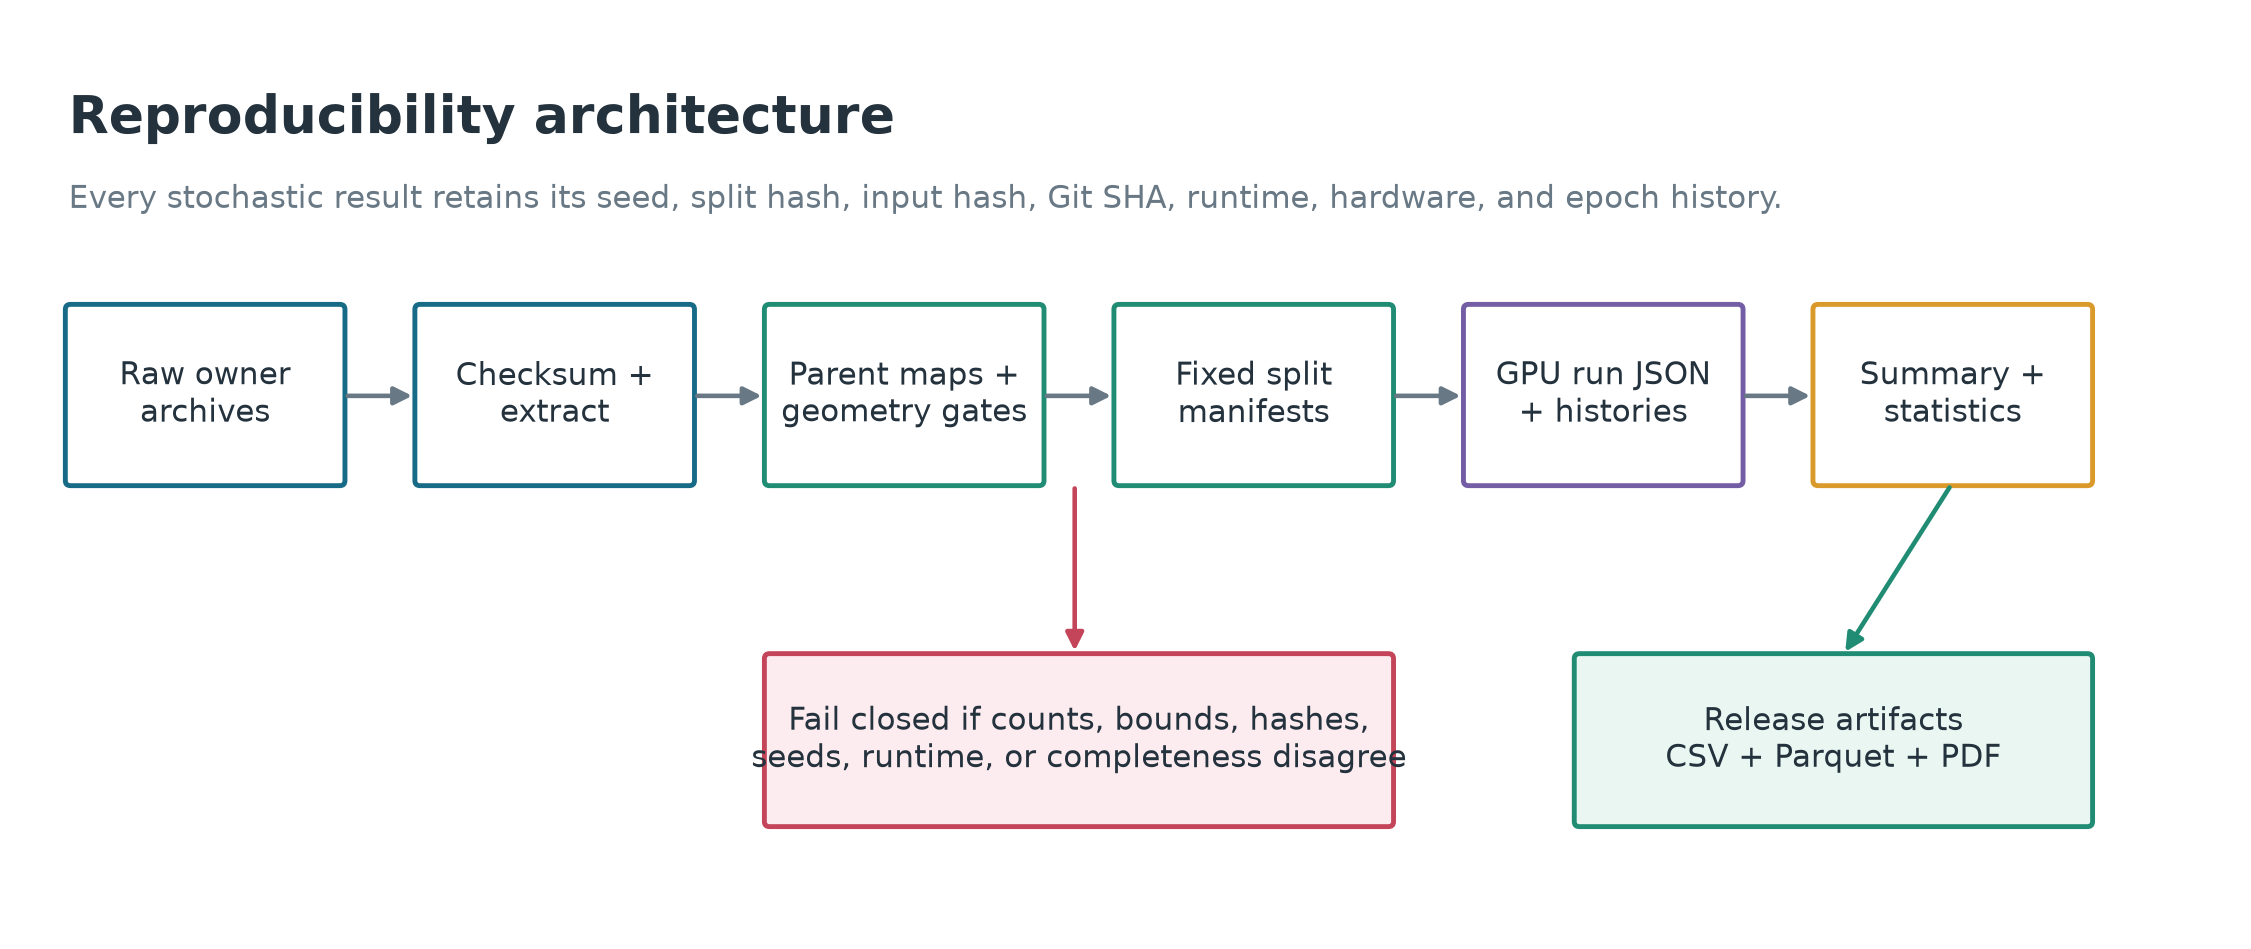
\includegraphics[width=\textwidth]{reproducibility_pipeline.png}
\caption{Reproducibility architecture. Deterministic provenance and split artifacts gate the stochastic GPU experiments, and every final result carries the hashes needed to reconnect it to its inputs.}
\label{s1:fig:repro-pipeline}
\end{figure}

The system deliberately separates three artifact layers:
\begin{enumerate}[leftmargin=2em]
  \item \textbf{Canonical identity:} exact or released parent IDs used to construct splits.
  \item \textbf{Independent audit:} image-matched parent IDs, boxes, confidence, runner-up margin, and an auxiliary diagnostic flag.
  \item \textbf{Sensitivity grouping:} P3 connected-component IDs built from thresholded cross-parent near-duplicate candidates.
\end{enumerate}

Keeping these layers separate prevents a lower-confidence image match from overwriting an exact filename identity. It also prevents a conservative pHash/dHash candidate from being narrated as a proven duplicate.

\section{Core artifact schemas}

The canonical SIPaKMeD map records \artifact{crop_id}, \artifact{parent_id}, \artifact{class_name}, paths, recovery method, and confidence. Branch B adds $x,y,w,h$, crop and parent dimensions, coarse and refined NCC, second-best confidence, margin, method, and diagnostic \artifact{accepted}. P3 adds \artifact{p3_group_id}. Split CSVs record \artifact{crop_id}, \artifact{parent_id}, \artifact{partition}, \artifact{protocol}, and \artifact{seed}.

Every neural result JSON records task, architecture, protocol/mode, seed, primary and secondary metrics, train/test counts, hyperparameters, exact split/input hashes, Git SHA, timestamps, elapsed time, visible GPU, platform and library versions, and full epoch history. This is more useful than a final number alone: it permits matrix completeness checks, runtime analysis, and learning-curve reconstruction without checkpoints.

\section{Fail-closed algorithm}

\begin{lstlisting}[style=cyto,caption={Conceptual fail-closed workflow.},label={lst:algorithm}]
for each released dataset:
    recover exact/released parent identity
    if an independent recovery branch exists:
        recover parent and bounding box without consulting branch A
        require >= 99% A/B agreement
    require one parent per observation
    require all boxes contained and all totals exact

construct P1, P1-prime, P2, and P3 for every fixed seed
measure structural and literal overlap
run probe/classifier/segmenter matrix with bounded GPUs

before summarizing:
    require every registered cell and seed exactly once
    require split hashes, runtime versions, and sample counts
    pair comparisons by seed
    attach an effect size and interval to every p-value
    apply BH over the entire declared family once

if any required evidence is absent:
    emit FAIL or PENDING; never infer PASS
\end{lstlisting}
